\documentclass[a4paper,11pt]{article}
\usepackage[utf8]{inputenc}
\usepackage[T1]{fontenc}
\usepackage{amsmath,amssymb}
\usepackage[a4paper,left=2cm,right=2cm,top=3.6cm,bottom=2.3cm,headheight=1.1cm,headsep=0.6cm,footskip=1cm]{geometry}
\usepackage{xcolor}
\usepackage{tikz}
\usetikzlibrary{calc,arrows.meta}
\usepackage{fancyhdr}
\usepackage{lastpage}
\usepackage{tabularx}
\usepackage{array}
\usepackage[most]{tcolorbox}
\usepackage{enumitem}
\usepackage{needspace}

\definecolor{navy}{HTML}{1F3A5F}
\definecolor{teal}{HTML}{0F8B7D}
\definecolor{softbg}{HTML}{F4F7FA}
\definecolor{brick}{HTML}{B03A2E}
\newcommand{\dis}{\displaystyle}

\setlength{\parindent}{0pt}
\renewcommand{\arraystretch}{1.35}

% ---------- header berwarna navy ----------
\pagestyle{fancy}
\fancyhf{}
\renewcommand{\headrulewidth}{0pt}
\fancyhead[L]{%
  \begin{tikzpicture}[remember picture,overlay]
    \fill[navy] ([yshift=-1.2cm]current page.north west) rectangle ([yshift=-3.15cm]current page.north east);
    \fill[teal] ([yshift=-3.15cm]current page.north west) rectangle ([yshift=-3.25cm]current page.north east);
  \end{tikzpicture}%
  \color{white}\bfseries\large Latihan Soal Fungsi Kuadrat}
\fancyhead[R]{\color{white}\small Diunduh dari website \textbf{Math1729}\ \,|\,\ 4 Oktober 2026}
\fancyfoot[L]{\small\color{navy}Math1729 --- Fungsi Kuadrat}
\fancyfoot[R]{\small\color{navy}Halaman \thepage\ dari \pageref{LastPage}}

% ---------- komponen ----------
\newcounter{no}
\newcommand{\bagian}[2]{\par\Needspace{6\baselineskip}\vspace{1.0em}\noindent
  \begin{tcolorbox}[colback=navy,colframe=navy,coltext=white,boxrule=0pt,arc=2pt,left=6pt,right=6pt,top=3pt,bottom=3pt]
  \textbf{#1}\hfill{\small #2}\end{tcolorbox}\setcounter{no}{0}\par\vspace{-0.3em}}
\newcommand{\tingkat}[2]{\par\Needspace{7\baselineskip}\vspace{0.6em}\noindent
  {\color{teal}\rule{3pt}{1.1em}}\ {\color{navy}\bfseries #1}\ {\small\color{gray}--- #2}\par\vspace{0.1em}}
\newcommand{\soal}[2]{\par\vspace{0.75em}\stepcounter{no}\noindent
  \begin{minipage}[t]{1.8em}\textbf{\theno.}\end{minipage}%
  \begin{minipage}[t]{\dimexpr\linewidth-1.8em\relax}#1\par\vspace{0.35em}#2\end{minipage}\par}
\newcommand{\poin}[1]{\hfill{\small\color{navy}[#1 poin]}}

% teks di kiri, gambar di kanan
\newcommand{\gbr}[2]{\noindent\begin{minipage}[t]{0.58\linewidth}#1\end{minipage}\hfill\raisebox{\ht\strutbox}{\begin{minipage}[t]{0.39\linewidth}\vspace{0pt}\centering#2\end{minipage}}}
\newcommand{\axs}[4]{\draw[-{Stealth[length=2mm]},thick] (#1,0)--(#3,0) node[right,font=\small]{$x$}; \draw[-{Stealth[length=2mm]},thick] (0,#2)--(0,#4) node[above,font=\small]{$y$};}

\begin{document}
\thispagestyle{fancy}

\begin{center}
  {\color{navy}\fontsize{22}{26}\selectfont\bfseries Latihan Soal Fungsi Kuadrat\par}
\end{center}
\vspace{2pt}
\begin{tcolorbox}[colback=softbg,colframe=navy!40,boxrule=0.6pt,arc=3pt,left=8pt,right=8pt,top=5pt,bottom=5pt]
\noindent\textbf{Nama} : \rule{4.6cm}{0.4pt}\hfill\textbf{Kelas} : \rule{2.2cm}{0.4pt}\hfill\textbf{Skor} : \rule{2.2cm}{0.4pt}
\end{tcolorbox}
\vspace{2pt}
\begin{tcolorbox}[colback=white,colframe=teal,boxrule=0.8pt,arc=3pt,left=8pt,right=8pt,top=4pt,bottom=4pt,title={\bfseries Petunjuk Pengerjaan},coltitle=white,fonttitle=\small]
\small
\begin{enumerate}[leftmargin=1.4em,itemsep=1pt,topsep=1pt]
\item Soal terdiri atas \textbf{20 pilihan ganda} (5 mudah, 5 sedang, 6 sulit, 4 HOTS), \textbf{5 isian singkat} (2 sedang, 3 sulit), dan \textbf{5 uraian (essay)} (4 sulit, 1 HOTS). Alokasi waktu yang disarankan: 120 menit.
\item Skor: pilihan ganda 2 poin, isian singkat 4 poin, uraian 8 poin per soal (total 100 poin). Tidak ada pengurangan skor untuk jawaban salah.
\item Untuk $f(x)=ax^{2}+bx+c$, diskriminan $D=b^{2}-4ac$. Grafik berada di atas sumbu-$x$ berarti $f(x)>0$. Gambar tidak selalu digambar sesuai skala.
\item Kalkulator tidak diperkenankan.
\end{enumerate}
\end{tcolorbox}

\bagian{A. Pilihan Ganda}{20 soal $\times$ 2 poin = 40 poin. Pilih satu jawaban yang paling tepat.}
\tingkat{Tingkat Mudah}{soal 1 sampai 5}
\soal{Jika $f(x)=2x^{2}-5x+3$, maka nilai $f(-1)$ adalah \dots.}{\begin{tabularx}{\linewidth}{@{}*{5}{X}@{}}\textbf{A.}\;$0$ & \textbf{B.}\;$4$ & \textbf{C.}\;$6$ & \textbf{D.}\;$10$ & \textbf{E.}\;$14$\end{tabularx}}
\soal{Himpunan penyelesaian persamaan $x^{2}+2x-15=0$ adalah \dots.}{\begin{tabularx}{\linewidth}{@{}*{5}{X}@{}}\textbf{A.}\;$\{-5,-3\}$ & \textbf{B.}\;$\{-5,3\}$ & \textbf{C.}\;$\{-3,5\}$ & \textbf{D.}\;$\{3,5\}$ & \textbf{E.}\;$\{-15,1\}$\end{tabularx}}
\soal{Persamaan sumbu simetri parabola $y=x^{2}-8x+10$ adalah \dots.}{\begin{tabularx}{\linewidth}{@{}*{5}{X}@{}}\textbf{A.}\;$x=-4$ & \textbf{B.}\;$x=2$ & \textbf{C.}\;$x=4$ & \textbf{D.}\;$x=8$ & \textbf{E.}\;$x=10$\end{tabularx}}
\soal{\gbr{Perhatikan grafik fungsi kuadrat pada gambar. Koordinat titik puncak grafik tersebut adalah \dots.}{%
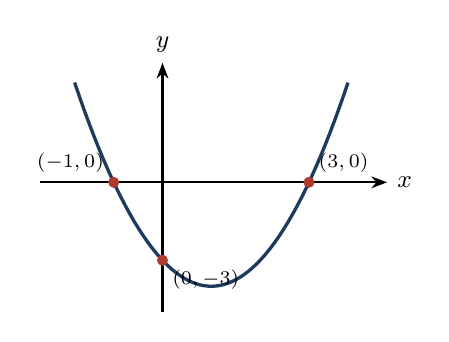
\begin{tikzpicture}[x=0.62cm,y=0.33cm]
\draw[very thick,navy,domain=-1.8:3.8,samples=60] plot ({\x},{\x*\x-2*\x-3});
\axs{-2.5}{-5}{4.6}{4.6}
\fill[brick] (-1,0) circle (2pt); \fill[brick] (3,0) circle (2pt); \fill[brick] (0,-3) circle (2pt);
\node[above left,font=\scriptsize] at (-1,0) {$(-1,0)$}; \node[above right,font=\scriptsize] at (3,0) {$(3,0)$};
\node[below right,font=\scriptsize] at (0,-3) {$(0,-3)$};
\end{tikzpicture}}}{\begin{tabularx}{\linewidth}{@{}*{5}{X}@{}}\textbf{A.}\;$(1,-4)$ & \textbf{B.}\;$(-1,-4)$ & \textbf{C.}\;$(1,-3)$ & \textbf{D.}\;$(2,-3)$ & \textbf{E.}\;$(3,0)$\end{tabularx}}
\soal{Persamaan kuadrat $2x^{2}-3x+5=0$ mempunyai diskriminan $D$ dengan pernyataan yang benar \dots.}{\begin{tabularx}{\linewidth}{@{}X@{}}\textbf{A.}\;$D=49$, dua akar real berbeda\\[1pt] \textbf{B.}\;$D=31$, dua akar real berbeda\\[1pt] \textbf{C.}\;$D=-31$, dua akar real berbeda\\[1pt] \textbf{D.}\;$D=-31$, dua akar real kembar\\[1pt] \textbf{E.}\;$D=-31$, tidak mempunyai akar real\end{tabularx}}
\tingkat{Tingkat Sedang}{soal 6 sampai 10}
\soal{Nilai minimum fungsi $f(x)=2x^{2}-12x+7$ adalah \dots.}{\begin{tabularx}{\linewidth}{@{}*{5}{X}@{}}\textbf{A.}\;$-25$ & \textbf{B.}\;$-18$ & \textbf{C.}\;$-11$ & \textbf{D.}\;$-7$ & \textbf{E.}\;$7$\end{tabularx}}
\soal{Grafik fungsi kuadrat memotong sumbu-$x$ di $(1,0)$ dan $(5,0)$ serta mempunyai nilai maksimum $8$. Persamaan fungsi tersebut adalah \dots.}{\begin{tabularx}{\linewidth}{@{}*{3}{X}@{}}\textbf{A.}\;$y=-2x^{2}+12x-10$ & \textbf{B.}\;$y=2x^{2}-12x+10$ & \textbf{C.}\;$y=-x^{2}+6x-5$\\[3pt] \textbf{D.}\;$y=-2x^{2}+12x-8$ & \textbf{E.}\;$y=-4x^{2}+24x-20$ & \end{tabularx}}
\soal{\gbr{Grafik fungsi kuadrat pada gambar mempunyai titik puncak $(-1,4)$ dan melalui titik $(0,3)$. Persamaan fungsinya adalah \dots.}{%
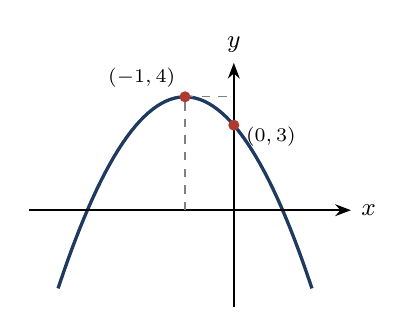
\begin{tikzpicture}[x=0.62cm,y=0.36cm]
\draw[very thick,navy,domain=-3.6:1.6,samples=60] plot ({\x},{-\x*\x-2*\x+3});
\axs{-4.2}{-3.4}{2.4}{5.2}
\draw[dashed,gray] (-1,0)--(-1,4); \draw[dashed,gray] (-1,4)--(0,4);
\fill[brick] (-1,4) circle (2pt); \fill[brick] (0,3) circle (2pt);
\node[above left,font=\scriptsize] at (-1,4) {$(-1,4)$}; \node[right,font=\scriptsize] at (0.05,2.6) {$(0,3)$};
\end{tikzpicture}}}{\begin{tabularx}{\linewidth}{@{}*{3}{X}@{}}\textbf{A.}\;$y=-x^{2}+2x+3$ & \textbf{B.}\;$y=x^{2}+2x+3$ & \textbf{C.}\;$y=-x^{2}-2x-3$\\[3pt] \textbf{D.}\;$y=-2x^{2}-4x+2$ & \textbf{E.}\;$y=-x^{2}-2x+3$ & \end{tabularx}}
\soal{Parabola $y=x^{2}-4x+1$ digeser $1$ satuan ke kiri dan $2$ satuan ke bawah. Persamaan parabola hasil pergeseran adalah \dots.}{\begin{tabularx}{\linewidth}{@{}*{5}{X}@{}}\textbf{A.}\;$y=x^{2}-6x+4$ & \textbf{B.}\;$y=x^{2}-2x$ & \textbf{C.}\;$y=x^{2}-4x-1$ & \textbf{D.}\;$y=x^{2}-2x-4$ & \textbf{E.}\;$y=x^{2}+2x-4$\end{tabularx}}
\soal{Akar-akar persamaan $x^{2}-8x+k=0$ adalah $x_{1}$ dan $x_{2}$. Jika $x_{1}=3x_{2}$, maka nilai $k$ adalah \dots.}{\begin{tabularx}{\linewidth}{@{}*{5}{X}@{}}\textbf{A.}\;$6$ & \textbf{B.}\;$12$ & \textbf{C.}\;$16$ & \textbf{D.}\;$18$ & \textbf{E.}\;$24$\end{tabularx}}
\tingkat{Tingkat Sulit}{soal 11 sampai 16, setara UTBK}
\soal{Garis $y=mx-1$ menyinggung parabola $y=x^{2}-4x+3$. Jumlah semua nilai $m$ yang memenuhi adalah \dots.}{\begin{tabularx}{\linewidth}{@{}*{5}{X}@{}}\textbf{A.}\;$-8$ & \textbf{B.}\;$-4$ & \textbf{C.}\;$0$ & \textbf{D.}\;$4$ & \textbf{E.}\;$8$\end{tabularx}}
\soal{Agar grafik $y=x^{2}+px+2$ seluruhnya berada di atas garis $y=2x-2$, nilai $p$ harus memenuhi \dots.}{\begin{tabularx}{\linewidth}{@{}*{3}{X}@{}}\textbf{A.}\;$-6<p<2$ & \textbf{B.}\;$-2<p<6$ & \textbf{C.}\;$p<-2$ atau $p>6$\\[3pt] \textbf{D.}\;$-4<p<4$ & \textbf{E.}\;$2<p<6$ & \end{tabularx}}
\soal{Grafik fungsi kuadrat $f$ melalui titik $(0,5)$, $(1,2)$, dan $(3,8)$. Nilai minimum $f$ adalah \dots.}{\begin{tabularx}{\linewidth}{@{}*{5}{X}@{}}\textbf{A.}\;$\dis\frac58$ & \textbf{B.}\;$\dis\frac54$ & \textbf{C.}\;$\dis\frac74$ & \textbf{D.}\;$\dis\frac{15}{8}$ & \textbf{E.}\;$\dis\frac{25}{8}$\end{tabularx}}
\soal{Jika $x$ dan $y$ bilangan real dengan $x+2y=10$, maka nilai minimum $x^{2}+y^{2}$ adalah \dots.}{\begin{tabularx}{\linewidth}{@{}*{5}{X}@{}}\textbf{A.}\;$10$ & \textbf{B.}\;$16$ & \textbf{C.}\;$20$ & \textbf{D.}\;$25$ & \textbf{E.}\;$40$\end{tabularx}}
\soal{Seorang peternak mempunyai kawat sepanjang $120$ m untuk membuat kandang berbentuk persegi panjang yang dibagi dua sama besar oleh sebuah sekat (sekat sejajar salah satu sisi dan memakai kawat juga). Luas total kandang terbesar yang mungkin adalah \dots\ m$^{2}$.}{\begin{tabularx}{\linewidth}{@{}*{5}{X}@{}}\textbf{A.}\;$150$ & \textbf{B.}\;$300$ & \textbf{C.}\;$400$ & \textbf{D.}\;$450$ & \textbf{E.}\;$600$\end{tabularx}}
\soal{Garis $y=2x+k$ memotong parabola $y=x^{2}-4x+5$ di titik $A$ dan $B$. Jika selisih absis $A$ dan $B$ adalah $6$, maka $k=$ \dots.}{\begin{tabularx}{\linewidth}{@{}*{5}{X}@{}}\textbf{A.}\;$1$ & \textbf{B.}\;$2$ & \textbf{C.}\;$3$ & \textbf{D.}\;$5$ & \textbf{E.}\;$9$\end{tabularx}}
\tingkat{Tingkat HOTS}{soal 17 sampai 20, penalaran tingkat tinggi}
\soal{\gbr{Perhatikan grafik fungsi $f(x)=ax^{2}+bx+c$ pada gambar, yang memotong sumbu-$x$ di $x=-3$ dan $x=-1$. Pernyataan yang benar adalah \dots.}{%
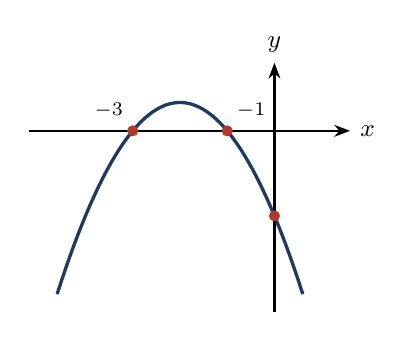
\begin{tikzpicture}[x=0.6cm,y=0.36cm]
\draw[very thick,navy,domain=-4.6:0.6,samples=60] plot ({\x},{-\x*\x-4*\x-3});
\axs{-5.2}{-6.4}{1.6}{2.4}
\fill[brick] (-3,0) circle (2pt); \fill[brick] (-1,0) circle (2pt); \fill[brick] (0,-3) circle (2pt);
\node[above left,font=\scriptsize] at (-3,0.1) {$-3$}; \node[above right,font=\scriptsize] at (-1,0.1) {$-1$};
\end{tikzpicture}}}{\begin{tabularx}{\linewidth}{@{}*{5}{X}@{}}\textbf{A.}\;$abc>0$ & \textbf{B.}\;$b^{2}-4ac<0$ & \textbf{C.}\;$a+b+c>0$ & \textbf{D.}\;$\dis\frac{b}{a}<0$ & \textbf{E.}\;$a-b+c=0$\end{tabularx}}
\soal{Fungsi $f(x)=x^{2}-2px+p+6$ mempunyai nilai minimum $m(p)$ untuk setiap bilangan real $p$. Nilai maksimum dari $m(p)$ adalah \dots.}{\begin{tabularx}{\linewidth}{@{}*{5}{X}@{}}\textbf{A.}\;$6$ & \textbf{B.}\;$\dis\frac{25}{4}$ & \textbf{C.}\;$\dis\frac{13}{2}$ & \textbf{D.}\;$7$ & \textbf{E.}\;$\dis\frac{25}{2}$\end{tabularx}}
\soal{Fungsi kuadrat $f$ memenuhi $f(1)=f(5)$, mempunyai nilai minimum $-4$, dan $f(0)=8$. Jika $x_{1}$ dan $x_{2}$ adalah akar-akar $f(x)=0$, maka $x_{1}^{2}+x_{2}^{2}=$ \dots.}{\begin{tabularx}{\linewidth}{@{}*{5}{X}@{}}\textbf{A.}\;$24$ & \textbf{B.}\;$30$ & \textbf{C.}\;$36$ & \textbf{D.}\;$42$ & \textbf{E.}\;$48$\end{tabularx}}
\soal{Banyak bilangan bulat $x$ yang memenuhi $\left|x^{2}-5x\right|<6$ adalah \dots.}{\begin{tabularx}{\linewidth}{@{}*{5}{X}@{}}\textbf{A.}\;$2$ & \textbf{B.}\;$3$ & \textbf{C.}\;$4$ & \textbf{D.}\;$5$ & \textbf{E.}\;$6$\end{tabularx}}
\bagian{B. Isian Singkat}{5 soal $\times$ 4 poin = 20 poin. Tuliskan hanya jawaban akhir.}
\tingkat{Tingkat Sedang}{soal 1 dan 2}
\soal{Grafik fungsi $f(x)=x^{2}+bx+c$ mempunyai titik puncak $(-3,-2)$. Nilai $b+c$ adalah \dots}{\hfill Jawaban: \rule{4.5cm}{0.4pt}}
\soal{Persamaan kuadrat $x^{2}-(m+2)x+9=0$ mempunyai dua akar real yang sama. Nilai $m$ yang positif adalah \dots}{\hfill Jawaban: \rule{4.5cm}{0.4pt}}
\tingkat{Tingkat Sulit}{soal 3 sampai 5}
\soal{Jika $\alpha$ dan $\beta$ adalah akar-akar persamaan $x^{2}-6x+4=0$, maka nilai $\sqrt{\alpha}+\sqrt{\beta}$ adalah \dots}{\hfill Jawaban: \rule{4.5cm}{0.4pt}}
\soal{Garis $y=3x+n$ menyinggung parabola $y=x^{2}-x+5$. Koordinat titik singgungnya adalah \dots}{\hfill Jawaban: \rule{4.5cm}{0.4pt}}
\soal{\gbr{Sebuah lengkungan jembatan berbentuk parabola dengan lebar dasar $40$ m dan tinggi bagian tengah $10$ m (lihat gambar). Tinggi lengkungan di titik yang berjarak $5$ m dari salah satu ujung dasarnya adalah \dots\ m.}{%
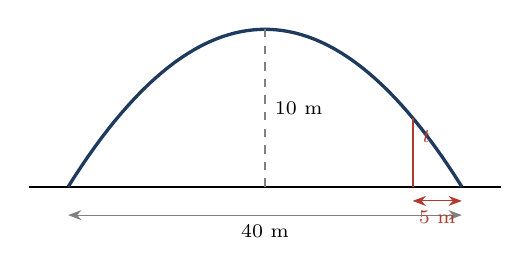
\begin{tikzpicture}[x=0.125cm,y=0.2cm]
\draw[thick] (-24,0)--(24,0);
\draw[very thick,navy,domain=-20:20,samples=60] plot ({\x},{10-\x*\x/40});
\draw[dashed,gray] (0,0)--(0,10); \node[right,font=\scriptsize] at (0,5) {$10$ m};
\draw[<->,>=Stealth,gray] (-20,-1.8)--(20,-1.8); \node[below,font=\scriptsize] at (0,-1.8) {$40$ m};
\draw[brick,thick] (15,0)--(15,4.375); \node[above right,font=\scriptsize,brick] at (15,2.2) {$t$};
\draw[<->,>=Stealth,brick] (15,-0.9)--(20,-0.9); \node[below,font=\scriptsize,brick] at (17.5,-0.9) {$5$ m};
\end{tikzpicture}}}{\hfill Jawaban: \rule{4.5cm}{0.4pt}}
\bagian{C. Uraian (Essay)}{5 soal $\times$ 8 poin = 40 poin. Tuliskan langkah penyelesaian dengan lengkap.}
\tingkat{Tingkat Sulit}{soal 1 sampai 4}
\soal{Diketahui persamaan kuadrat $x^{2}-(m+1)x+m+4=0$.\par\smallskip(a) Tentukan batas nilai $m$ agar persamaan mempunyai dua akar real yang berbeda.\par(b) Tentukan batas nilai $m$ agar kedua akarnya real dan positif.\par(c) Jika akar-akarnya $x_{1},x_{2}$ real berbeda dan $x_{1}^{2}+x_{2}^{2}=18$, tentukan nilai $m$.}{\poin{8}}
\soal{\gbr{Parabola $y=x^{2}-6x+5$ memotong sumbu-$x$ di titik $A$ dan $B$, memotong sumbu-$y$ di titik $D$, dan mempunyai titik puncak $C$ (lihat gambar).\par\smallskip(a) Tentukan koordinat $A$, $B$, dan $C$.\par(b) Hitung luas segitiga $ABC$.\par(c) Tentukan persamaan garis yang melalui $C$ dan $D$.}{%
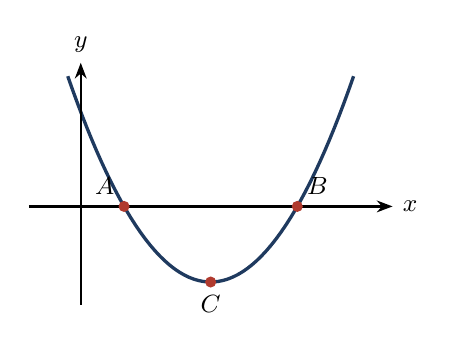
\begin{tikzpicture}[x=0.55cm,y=0.24cm]
\draw[very thick,navy,domain=-0.3:6.3,samples=60] plot ({\x},{\x*\x-6*\x+5});
\axs{-1.2}{-5.2}{7.2}{7.6}
\fill[brick] (1,0) circle (2pt); \fill[brick] (5,0) circle (2pt); \fill[brick] (3,-4) circle (2pt);
\node[above left,font=\small] at (1,0.1) {$A$}; \node[above right,font=\small] at (5,0.1) {$B$}; \node[below,font=\small] at (3,-4.2) {$C$};
\end{tikzpicture}}}{\poin{8}}
\soal{Sebuah toko menjual kaus dengan harga Rp80.000 per buah dan terjual $200$ buah per bulan. Setiap kenaikan harga Rp5.000, penjualan turun $10$ buah per bulan. Misal $x$ adalah banyak kenaikan harga sebesar Rp5.000.\par\smallskip(a) Nyatakan pendapatan bulanan $R(x)$ dalam $x$ (dalam ribu rupiah).\par(b) Tentukan harga jual agar pendapatan maksimum, beserta pendapatan maksimumnya.\par(c) Jika biaya pengadaan Rp50.000 per kaus, tentukan harga jual agar laba bulanan maksimum.}{\poin{8}}
\soal{Diketahui parabola $y=x^{2}-4x+6$ dan garis $y=2x+k$.\par\smallskip(a) Tentukan nilai $k$ agar garis menyinggung parabola, lalu tentukan titik singgungnya.\par(b) Tentukan batas nilai $k$ agar garis memotong parabola di dua titik berbeda.\par(c) Untuk $k=-2$, tentukan koordinat kedua titik potong dan jarak antara keduanya.}{\poin{8}}
\tingkat{Tingkat HOTS}{soal 5}
\soal{Diketahui fungsi $f(x)=x^{2}-2(p-1)x+p^{2}-3p$ dengan $p$ bilangan real.\par\smallskip(a) Tentukan koordinat titik puncak grafik $f$ dinyatakan dalam $p$.\par(b) Buktikan bahwa untuk setiap nilai $p$, titik puncak grafik $f$ terletak pada satu garis lurus yang sama, lalu tentukan persamaan garis tersebut.\par(c) Tentukan nilai $p$ agar grafik $f$ menyinggung sumbu-$x$, lalu tentukan titik singgungnya.}{\poin{8}}
\newpage
\bagian{Kunci Jawaban dan Pembahasan Singkat}{Untuk guru dan pembahasan mandiri}
\par\vspace{0.6em}{\bfseries\color{navy}Kunci Pilihan Ganda}\par\vspace{0.3em}
\begin{tabularx}{\linewidth}{@{}*{10}{>{\centering\arraybackslash}X}@{}}\hline \textbf{1} & \textbf{2} & \textbf{3} & \textbf{4} & \textbf{5} & \textbf{6} & \textbf{7} & \textbf{8} & \textbf{9} & \textbf{10}\\ \hline D & B & C & A & E & C & A & E & D & B\\ \hline\end{tabularx}\par\vspace{0.4em}\begin{tabularx}{\linewidth}{@{}*{10}{>{\centering\arraybackslash}X}@{}}\hline \textbf{11} & \textbf{12} & \textbf{13} & \textbf{14} & \textbf{15} & \textbf{16} & \textbf{17} & \textbf{18} & \textbf{19} & \textbf{20}\\ \hline A & B & D & C & E & D & E & B & A & C\\ \hline\end{tabularx}
\par\vspace{0.8em}{\bfseries\color{navy}Pembahasan Pilihan Ganda}\par\vspace{0.2em}
\small\begin{enumerate}[leftmargin=2em,itemsep=2pt,topsep=2pt]
\item[\textbf{1.}] \textbf{(D)} $f(-1)=2(1)-5(-1)+3=2+5+3=10$.
\item[\textbf{2.}] \textbf{(B)} $x^{2}+2x-15=(x+5)(x-3)=0\Rightarrow x=-5$ atau $x=3$.
\item[\textbf{3.}] \textbf{(C)} Sumbu simetri $x=-\dis\frac{b}{2a}=-\dis\frac{-8}{2}=4$.
\item[\textbf{4.}] \textbf{(A)} Titik potong sumbu-$x$ di $-1$ dan $3$, sehingga sumbu simetri $x=\dis\frac{-1+3}{2}=1$. Grafik melalui $(0,-3)$ dengan $f(x)=a(x+1)(x-3)$: $-3=a(1)(-3)\Rightarrow a=1$. Maka $f(1)=1\cdot2\cdot(-2)=-4$, puncaknya $(1,-4)$.
\item[\textbf{5.}] \textbf{(E)} $D=b^{2}-4ac=(-3)^{2}-4(2)(5)=9-40=-31<0$, sehingga persamaan tidak mempunyai akar real.
\item[\textbf{6.}] \textbf{(C)} Absis puncak $x=-\dis\frac{-12}{4}=3$, sehingga $f(3)=2(9)-36+7=-11$. (Atau $-\dis\frac{D}{4a}=-\dis\frac{144-56}{8}=-11$.)
\item[\textbf{7.}] \textbf{(A)} $y=a(x-1)(x-5)$ dengan sumbu simetri $x=3$. Nilai maksimum: $a(2)(-2)=8\Rightarrow a=-2$. Maka $y=-2(x^{2}-6x+5)=-2x^{2}+12x-10$.
\item[\textbf{8.}] \textbf{(E)} $y=a(x+1)^{2}+4$. Melalui $(0,3)$: $3=a+4\Rightarrow a=-1$. Maka $y=-(x+1)^{2}+4=-x^{2}-2x+3$.
\item[\textbf{9.}] \textbf{(D)} Puncak semula $(2,-3)$. Setelah digeser menjadi $(1,-5)$ dengan $a=1$ tetap: $y=(x-1)^{2}-5=x^{2}-2x-4$. (Cek: ganti $x$ dengan $x+1$ dan kurangi $2$.)
\item[\textbf{10.}] \textbf{(B)} $x_{1}+x_{2}=8\Rightarrow4x_{2}=8\Rightarrow x_{2}=2,\ x_{1}=6$. Maka $k=x_{1}x_{2}=12$.
\item[\textbf{11.}] \textbf{(A)} $x^{2}-4x+3=mx-1\Rightarrow x^{2}-(m+4)x+4=0$. Menyinggung: $D=0\Rightarrow(m+4)^{2}=16\Rightarrow m=0$ atau $m=-8$. Jumlahnya $-8$.
\item[\textbf{12.}] \textbf{(B)} $x^{2}+px+2>2x-2\Rightarrow x^{2}+(p-2)x+4>0$ untuk semua $x$. Syarat $D<0$: $(p-2)^{2}-16<0\Rightarrow-4<p-2<4\Rightarrow-2<p<6$.
\item[\textbf{13.}] \textbf{(D)} $f(x)=ax^{2}+bx+c$: $c=5$; $a+b+5=2\Rightarrow a+b=-3$; $9a+3b+5=8\Rightarrow3a+b=1$. Maka $a=2,\ b=-5$, $f(x)=2x^{2}-5x+5$. Nilai minimum $=5-\dis\frac{25}{8}=\dis\frac{15}{8}$.
\item[\textbf{14.}] \textbf{(C)} $x=10-2y\Rightarrow x^{2}+y^{2}=(10-2y)^{2}+y^{2}=5y^{2}-40y+100$. Minimum di $y=4$: $5(16)-160+100=20$.
\item[\textbf{15.}] \textbf{(E)} Misal panjang sisi sejajar sekat $L$ dan sisi lainnya $W$. Kawat: $3L+2W=120\Rightarrow W=\dis\frac{120-3L}{2}$. Luas $=L\cdot W=\dis\frac{120L-3L^{2}}{2}$, maksimum di $L=20$: $\dis\frac{2400-1200}{2}=600$ m$^{2}$.
\item[\textbf{16.}] \textbf{(D)} $x^{2}-4x+5=2x+k\Rightarrow x^{2}-6x+(5-k)=0$. Selisih akar $|x_{1}-x_{2}|=\dis\frac{\sqrt D}{a}=\sqrt{36-4(5-k)}=\sqrt{16+4k}=6\Rightarrow16+4k=36\Rightarrow k=5$.
\item[\textbf{17.}] \textbf{(E)} Grafik terbuka ke bawah ($a<0$), memotong sumbu-$y$ di bawah sumbu-$x$ ($c<0$), dan kedua akar negatif sehingga $-\dis\frac ba<0\Rightarrow\dis\frac ba>0\Rightarrow b<0$. Maka $abc<0$ (A salah), $D>0$ (B salah), $f(1)=a+b+c<0$ (C salah), $\dis\frac ba>0$ (D salah). Karena $x=-1$ adalah akar, $f(-1)=a-b+c=0$ (E benar).
\item[\textbf{18.}] \textbf{(B)} Puncak di $x=p$, sehingga $m(p)=f(p)=p^{2}-2p^{2}+p+6=-p^{2}+p+6$. Ini parabola terbuka ke bawah dengan maksimum di $p=\dis\frac12$: $m=-\dis\frac14+\dis\frac12+6=\dis\frac{25}{4}$.
\item[\textbf{19.}] \textbf{(A)} $f(1)=f(5)\Rightarrow$ sumbu simetri $x=3$, puncak $(3,-4)$: $f(x)=a(x-3)^{2}-4$. Dari $f(0)=8$: $9a-4=8\Rightarrow a=\dis\frac43$. Maka $f(x)=0\Rightarrow(x-3)^{2}=3\Rightarrow x=3\pm\sqrt3$. $x_{1}^{2}+x_{2}^{2}=(x_1+x_2)^2-2x_1x_2=6^{2}-2(6)=24$.
\item[\textbf{20.}] \textbf{(C)} $-6<x^{2}-5x<6$. Dari $x^{2}-5x-6<0$: $-1<x<6$. Dari $x^{2}-5x+6>0$: $x<2$ atau $x>3$. Irisan: $-1<x<2$ atau $3<x<6$. Bilangan bulatnya $0,1,4,5$, yaitu $4$ bilangan.
\end{enumerate}
\par\Needspace{6\baselineskip}\vspace{0.6em}{\bfseries\color{navy}\normalsize Pembahasan Isian Singkat}\par\vspace{0.2em}
\small\begin{enumerate}[leftmargin=2em,itemsep=2pt,topsep=2pt]
\item[\textbf{1.}] \textbf{Jawaban: $13$.} $f(x)=(x+3)^{2}-2=x^{2}+6x+7\Rightarrow b=6,\ c=7$, sehingga $b+c=13$.
\item[\textbf{2.}] \textbf{Jawaban: $4$.} Akar kembar: $D=0\Rightarrow(m+2)^{2}-36=0\Rightarrow m+2=\pm6\Rightarrow m=4$ atau $m=-8$. Yang positif: $m=4$.
\item[\textbf{3.}] \textbf{Jawaban: $\sqrt{10}$.} $\alpha+\beta=6$ dan $\alpha\beta=4$ (kedua akar positif). $\left(\sqrt\alpha+\sqrt\beta\right)^{2}=\alpha+\beta+2\sqrt{\alpha\beta}=6+2\cdot2=10$, sehingga $\sqrt\alpha+\sqrt\beta=\sqrt{10}$.
\item[\textbf{4.}] \textbf{Jawaban: $(2,7)$.} $x^{2}-x+5=3x+n\Rightarrow x^{2}-4x+(5-n)=0$. Menyinggung: $D=16-4(5-n)=0\Rightarrow n=1$. Akar ganda $x=2$, $y=3(2)+1=7$. Titik singgung $(2,7)$.
\item[\textbf{5.}] \textbf{Jawaban: $4{,}375$ m.} Pasang sumbu di tengah dasar: $y=10-kx^{2}$ dengan $y=0$ di $x=20$: $400k=10\Rightarrow k=\dis\frac1{40}$. Titik berjarak $5$ m dari ujung berada di $x=15$: $y=10-\dis\frac{225}{40}=\dis\frac{35}{8}=4{,}375$ m.
\end{enumerate}
\par\Needspace{8\baselineskip}\vspace{0.6em}{\bfseries\color{navy}\normalsize Pembahasan dan Pedoman Penskoran Uraian}\par\vspace{0.2em}
\small\begin{enumerate}[leftmargin=2em,itemsep=3pt,topsep=2pt]
\item[\textbf{1.}] (a) $D=(m+1)^{2}-4(m+4)=m^{2}-2m-15=(m-5)(m+3)>0\Rightarrow m<-3$ atau $m>5$. (b) Real: $D\ge0\Rightarrow m\le-3$ atau $m\ge5$. Positif: $x_1+x_2=m+1>0\Rightarrow m>-1$ dan $x_1x_2=m+4>0\Rightarrow m>-4$. Irisan: $m\ge5$. (c) $x_1^2+x_2^2=(m+1)^2-2(m+4)=m^2-7=18\Rightarrow m=\pm5$. Dari (a), $m=5$ memberi $D=0$ (akar kembar, ditolak), sehingga $m=-5$. \\ \textit{Penskoran: Bagian (a) 2 poin; (b) 3 poin; (c) 3 poin.}
\item[\textbf{2.}] (a) $x^{2}-6x+5=(x-1)(x-5)=0$ memberi $A(1,0)$, $B(5,0)$. Puncak: $x=3$, $y=9-18+5=-4$, jadi $C(3,-4)$. (b) Alas $AB=4$, tinggi $=|-4|=4$, luas $=\dis\frac12\cdot4\cdot4=8$ satuan luas. (c) $D(0,5)$. Gradien $CD=\dis\frac{5-(-4)}{0-3}=-3$, sehingga $y-5=-3x\Rightarrow y=-3x+5$. (Cek $C$: $-9+5=-4$.) \\ \textit{Penskoran: Bagian (a) 3 poin; (b) 2 poin; (c) 3 poin.}
\item[\textbf{3.}] (a) Harga $=80+5x$ (ribu), terjual $=200-10x$. $R(x)=(80+5x)(200-10x)=16.000+200x-50x^{2}$. (b) Puncak di $x=-\dis\frac{200}{2(-50)}=2$: harga Rp90.000, $R(2)=16.200$ ribu $=$ Rp16.200.000. (c) Laba $L(x)=(80+5x-50)(200-10x)=(30+5x)(200-10x)=6.000+700x-50x^{2}$, maksimum di $x=-\dis\frac{700}{-100}=7$: harga $80+35=115$ ribu, yaitu Rp115.000 (laba maksimum $L(7)=8.450$ ribu $=$ Rp8.450.000). \\ \textit{Penskoran: Bagian (a) 2 poin; (b) 3 poin; (c) 3 poin.}
\item[\textbf{4.}] Substitusi: $x^{2}-4x+6=2x+k\Rightarrow x^{2}-6x+(6-k)=0$ dengan $D=36-4(6-k)=12+4k$. (a) Menyinggung: $D=0\Rightarrow k=-3$. Akar ganda $x=3$, $y=9-12+6=3$, titik singgung $(3,3)$. (b) Dua titik: $D>0\Rightarrow k>-3$. (c) $k=-2$: $x^{2}-6x+8=0\Rightarrow x=2$ atau $x=4$; titik $(2,2)$ dan $(4,6)$. Jarak $=\sqrt{(4-2)^{2}+(6-2)^{2}}=\sqrt{20}=2\sqrt5$. \\ \textit{Penskoran: Bagian (a) 3 poin; (b) 2 poin; (c) 3 poin.}
\item[\textbf{5.}] (a) Absis puncak $x=p-1$. Ordinat $f(p-1)=(p-1)^{2}-2(p-1)^{2}+p^{2}-3p=-(p-1)^{2}+p^{2}-3p=-p-1$. Puncak $(p-1,\,-p-1)$. (b) Misal $X=p-1$ dan $Y=-p-1$. Maka $p=X+1\Rightarrow Y=-(X+1)-1=-X-2$. Jadi semua puncak terletak pada garis $y=-x-2$. (c) Menyinggung sumbu-$x$: ordinat puncak $0\Rightarrow-p-1=0\Rightarrow p=-1$. Fungsi menjadi $x^{2}+4x+4=(x+2)^{2}$, titik singgung $(-2,0)$. \\ \textit{Penskoran: Bagian (a) 2 poin; (b) 3 poin; (c) 3 poin.}
\end{enumerate}
\end{document}